\section{Manage Users}
This chapter provides details about user and role management which you can
do if you have \emph{administrator} role. \emph{Manage Users} option from
\emph{Admin} menu will take you to the user list page (see Figure~\ref{fig:userlist}) 
from where you can: add new user(s) (one by one or bulk), view, edit,
enable/disable and delete users.
\subsection{Add Users}
To add a new user click on the \emph{Add}
button\footnote{Please note that newly added users need not to have AD account
before hand}.

\begin{figure}[hb!]
\centering
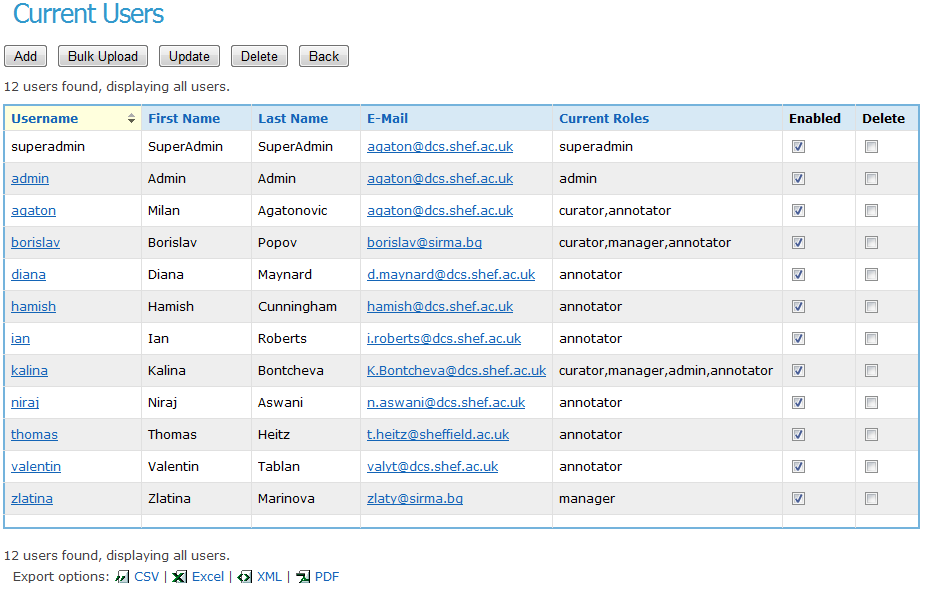
\includegraphics[scale=0.4]{userlist}
\caption{User List}
\label{fig:userlist}
\end{figure}

\subsection{Bulk Users Upload}
To upload multiple users click on
the \emph{Bulk Upload} button.
\begin{figure}[hb!]
\centering
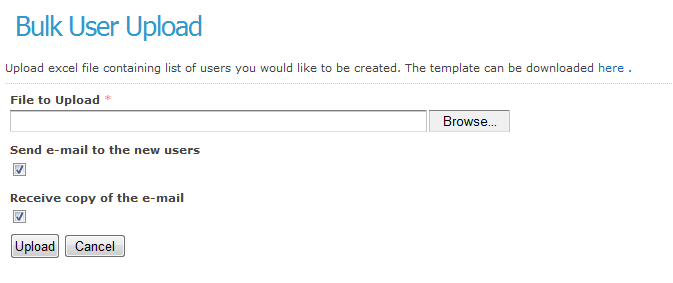
\includegraphics[scale=0.4]{bulkuserupload}
\caption{Bulk Users Upload}
\label{fig:bulkuserupload}
\end{figure}
You can download the excel template file, by clicking on provided link and fill
it with the user data like shown in
Figure~\ref{fig:bulkuseruploadxlstemplate}
If you want users to be notified upon their registration, check \emph{Send
e-mail to the new users}, and if you want yourself to have copy of this email
check \emph{Receive copy of the e-mail}.

\begin{figure}[hb!]
\centering
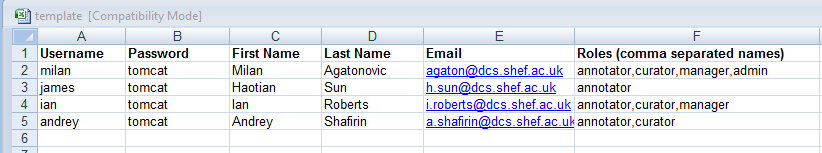
\includegraphics[scale=0.4]{bulkuseruploadxlstemplate}
\caption{Excel Template File}
\label{fig:bulkuseruploadxlstemplate}
\end{figure}

Please note that roles assigned to the new user have to comma separated

\subsection{View/Edit user profiles and roles}
If you want to update the information of the user
\emph{agaton}, he/she can simply click on the username link of
\emph{agaton} shown in Figure~\ref{fig:userlist}.

\begin{figure}[hb!]
\centering
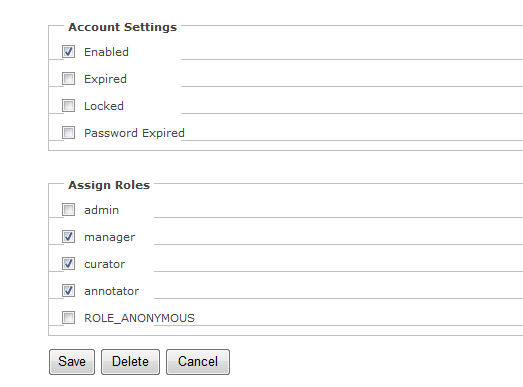
\includegraphics[scale=0.4]{userprofile}
\caption{Edit User Profile}
\label{fig:userprofile}
\end{figure}

The user information form will be displayed. In addition to the information
shown in Figure~\ref{fig:editprofile} previously, this form will be extended
to include details of user roles and account settings as shown in
Figure~\ref{fig:userprofile}. Here administrator can assign multiple
roles to each user.

\subsection{Enable/Disable Users}
You can quickly enable/disable multiple users by
ticking/unticking the checkboxes in the user list \emph{Enabled}, and clicking
on the \emph{Update} button.

\subsection{Delete Users}
You can delete multiple users by
ticking the checkboxes in the user list \emph{Delete} column, and
clicking on the \emph{Delete} button.

\section{Active users}
Who among users is online can be seen from the \emph{Active Users} page as
shown in Figure~\ref{fig:currentuser}.
\begin{figure}[hb!]
\centering
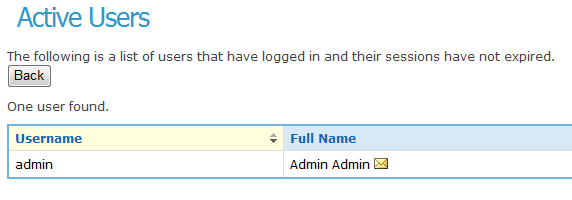
\includegraphics[scale=0.4]{currentuser}
\caption{Active Users}
\label{fig:currentuser}
\end{figure}

\section{Clickstreams}
Administrator can view user request history via \emph{Clickstreams} page, which 
is the last item in the Administration menu, as
shown in Figure~\ref{fig:allclickstreams}.
\begin{figure} [hb!]
\centering

\includegraphics[scale=0.5]{allclickstreams}
\caption{Clickstreams}
\label{fig:allclickstreams}
\end{figure}
